\chapter{晶格振动和声子}\label{chap:phonon}

在本章中我们需要考虑晶格的变形,因此,$\vb*{R}_{\vb*{i}}$不再是简单的$\vb*{i}$以初基格矢为基矢量张成的矢量,而会在此基础上有小的偏离。
使用$\vb*{R}^{(0)}$表示其它章节中的$\vb*{i}$以初基格矢为基矢量张成的$\vb*{R}_{\vb*{i}}$。

\section{举例:谐振子链导出的自由声子}

\subsection{一维简谐振子链}

首先考虑一个一维的、均质的晶格,并假定非线性效应很微弱,即不存在声子-声子散射,从而
\begin{equation}
    {H} = \sum_n \frac{{P}_n^2}{2 M} + \frac{M}{2} \sum_{n} \omega^2 ({X}_{n+1} - {X}_{n})^2.
    \label{eq:one-dim-osc-hamiltonian}
\end{equation}
记晶格常数为$a$,做傅里叶变换
\[
    {P}_n = \frac{1}{\sqrt{N}} \sum_{k} \ee^{\ii k n a} {P}_k, \quad {X}_n = \frac{1}{\sqrt{N}} \sum_{k} \ee^{\ii k n a} {X}_k,
\]
由于$\vb*{X}$和$\vb*{P}$都是实场,将$k$换成$-k$只会导致共轭转置。
可以计算出对易关系
\begin{equation}
    \comm*{{X}_{k}}{{P}_{k'}} = \ii \delta_{k+k', 0}, \quad \comm*{{X}_{k}}{{X}_{k'}} = \comm*{{P}_{k}}{{P}_{k'}} = 0,
\end{equation}
并将哈密顿量写成
\[
    {H} = \frac{1}{2M} \sum_{k} {P}_{-k} {P}_{k} + \sum_k \frac{M \omega_{k}}{2} {X}_{-k} {X}_k,
\]
其中
\begin{equation}
    \omega_k^2 = 2 (1 - \cos k a) \omega_0^2, \quad \omega_k > 0.
\end{equation}
做变换
\begin{equation}
    {b}_{k} = \sqrt{\frac{M \omega_k}{2}} {X}_k + \ii \frac{1}{\sqrt{2 M \omega_k}} P_k, \quad {b}^\dagger_{k} = \sqrt{\frac{M \omega_k}{2}} {X}_k - \ii \frac{1}{\sqrt{2 M \omega_k}} P_k,
\end{equation}
则有
\begin{equation}
    {H} = \sum_k \omega_k \left({b}^\dagger_k {b}_k + \frac{1}{2}\right).
\end{equation}
这样就得到了声子。

另一种更加一般的方法是傅里叶变换。% TODO
注意此时$\omega$表面上看有两个解,一正一负,但是因为$\vb*{X}$是实场,其正频部分和负频部分不是独立的,即所谓“增加一个频率为$-\omega$的声子”就是“消灭一个频率为$\omega$的声子”。
因此,只需要取$\omega > 0$的情况,就覆盖了所有的声子模式。
用场论的话说,声子由于是实场的量子化产生的,其反粒子就是声子。

\begin{back}{反粒子}{anti-particles}
    设已有粒子产生算符$a^\dagger$,取其复共轭$b^\dagger = a$,会发现$b$粒子的能量正好是$a$粒子的能量的相反数;此外为了保证动量守恒(自行写一个顶角验证即可),我们会发现$a^\dagger_{\vb*{k}} = b_{- \vb*{k}}$。
    我们称$b$粒子为$a$粒子的\concept{反粒子}。在规范场论中一种粒子的荷和它的反粒子也相反。
    但是反粒子和粒子的质量和自旋是一样的。

    一个复场的量子化会产生两种粒子,彼此互为反粒子,但是一个实场产生的粒子的反粒子实际上就是它自身,即$a^\dagger_{\vb*{k}} = a_{- \vb*{k}}$。
\end{back}

\subsection{三维单成分正方晶格}

现在考虑一个三维的正方晶格,各个离子实还是一模一样的。用下标标记晶格坐标,用上标标记矢量的分量,得到\eqref{eq:one-dim-osc-hamiltonian}的三维版本(已经略去了一个无关紧要的基态能量$V_0$):
\begin{equation}
    {H} = \frac{1}{2 M} \sum_{\vb*{i}} {P}_{\vb*{i}}^2 + \frac{1}{2} \sum_{\pair{\vb*{i}, \vb*{j}}} \pdv{V}{R^a}{R^b} (X_{\vb*{i}}^a - X_{\vb*{j}}^a) (X_{\vb*{i}}^b - X_{\vb*{j}}^b).
\end{equation}
将$\vb*{X}_{\vb*{i}}$和$\vb*{P}_{\vb*{i}}$做如下展开:
\begin{equation}
    \vb*{X}_{\vb*{i}} = \frac{1}{\sqrt{N}} \sum_{\vb*{k}, \lambda} \vb*{\lambda} X_{\vb*{i} \lambda} \ee^{\ii \vb*{k} \cdot \vb*{R}_{\vb*{i}}^0}, \quad \vb*{P}_{\vb*{i}} = \frac{1}{\sqrt{N}} \sum_{\vb*{k}, \lambda} \vb*{\lambda} P_{\vb*{i} \lambda} \ee^{\ii \vb*{k} \cdot \vb*{R}_{\vb*{i}}^0},
\end{equation}
其中$\vb*{\lambda}$是对称矩阵$\pdv{V}{R^a}{R^b}$的特征方向,我们用它表示不同的偏振方向(由于$\vb*{X}$是矢量,声子会有一个额外的偏振自由度)。
在系统对称性比较好的时候,无论$\vb*{k}$方向如何,都可以找到三个合适的$\vb*{\lambda}$,一个平行于$\vb*{k}$,两个垂直于$\vb*{k}$,即可以区分出明确的纵波模式和横波模式,从而可以对不同的$\vb*{k}$选取不同的$\vb*{\lambda}$,记作$\vb*{\lambda}_{\vb*{k}}$。
这样,哈密顿量就是
\begin{equation}
    {H} = \frac{1}{2 M} \sum_{\vb*{k}, \lambda} {P}_{-\vb*{k} \lambda} {P}_{\vb*{k}\lambda} + \frac{M}{2} \sum_{\vb*{k}, \lambda} \omega_{\vb*{k} \lambda}^2 {X}_{-\vb*{k} \lambda} {X}_{\vb*{k} \lambda}.
\end{equation}
容易看出,由于${H}$的厄米性,$\omega_{\vb*{k}\vb*{\lambda}} = \omega_{-\vb*{k} \vb*{\lambda}}$。做变换
\begin{equation}
    {b}_{\vb*{k} \lambda} = \sqrt{\frac{M \omega_{\vb*{k} \lambda}}{2}} {X}_{\vb*{k} \lambda} + \ii \frac{1}{\sqrt{2 M \omega_{\vb*{k} \lambda}}} P_{\vb*{k} \lambda}, \quad {b}^\dagger_{\vb*{k} \lambda} = \sqrt{\frac{M \omega_{\vb*{k} \lambda}}{2}} {X}_{- \vb*{k} \lambda} - \ii \frac{1}{\sqrt{2 M \omega_{\vb*{k} \lambda}}} P_{- \vb*{k} \lambda},
    \label{eq:transform-b-pq}
\end{equation}
哈密顿量就成为
\begin{equation}
    {H} = \sum_{\vb*{k}, \lambda} \omega_{\vb*{k} \lambda} \left( {b}^\dagger_{\vb*{k} \lambda} {b}_{\vb*{k} \lambda} + \frac{1}{2} \right).
\end{equation}

\section{理想晶体中声子的一般理论}

\subsection{声学声子和光学声子}

如果晶格是复式晶格,那么$\vb*{X}$需要两个量子数来标记,其一是格点坐标,其二是表明它是哪种原子的位移的一个标签。
这样,如果晶格有$n_\text{i}$种原子,那么它就有$3n_\text{i} N$个自由度,因子$3$来自三个振动方向;$N$个原胞在哈密顿量对角化后转化为连续的Bloch波矢,因此做完正则量子化之后,这$3n_\text{i} N$个自由度会产生$3n_\text{i}$条连续的声子能带或者说\concept{声子谱}。

如果晶格中只有一种原子,那么显然只有$3$条谱。另一方面Goldstone定理预言了由于连续平移对称性的破缺,一定会出现三个模式,那么这三个模式就是前述的那三个模式,并且这些模式在动量很小时色散关系近似为线性的。

声子作为一种准粒子,当然也服从\autoref{sec:quasi-particle-spectrum}中的说法,其“动量”也是局限在第一布里渊区中的。
一个复式的晶格可以看成单式晶格加入扰动之后的结果。我们将扰动视为微扰,从而获得复式晶格的声子谱的一些定性性质。
首先,扰动会让晶格的对称性下降,从而实空间中晶格常数增大,从而第一布里渊区缩小,即产生所谓布里渊区折叠%
\footnote{
    我们还会不止一次看到布里渊区折叠现象出现,在这里,布里渊区折叠是来自我们设定的扰动,而在一些低温电子配对情况下布里渊区折叠是自发出现的。
}%
。于是,类似于\autoref{fig:bloch-energy-band}的现象会出现在声子谱上,出现“声子能带”,一些声子模式变得有能隙,当然还有一些声子模式是无能隙的。
但是,Goldstone模式——在动量很小时色散关系为线性,没有能隙——还是只有那三个,我们称这些模式为\concept{声学声子},将剩下的$3n-3$个模式称为\concept{光学声子}。
显然,在长波极限下——即这个动量的声子足够多时,足以在宏观上产生效应的情况下——声子退化为固体力学振动,即声波,因为晶体中的宏观弹性波当然来自晶格振动,通过弹性力学的论证会发现它们的色散关系是线性的,并且宏观弹性波的频率通常都很低,因此三种弹性波或者说声波确实就是三个声学声子支。
由于不同的声子模式彼此解耦(或者至少,相互作用足够弱),三个方向上的声波应该能够对应到单一的声子模式上。
容易看出,它们只可能对应到声学声子上,这就是“声学声子”这个名称的由来。
另一方面,由于光学声子不对应弹性波,光学声子即使很多,也不会导致固体出现宏观的形变(但这不代表没有和光学声子对应的宏观场——比如说后面所说的电子密度就可以,光学声子的经典极限称为\concept{光学波}),但是此时一个晶胞中的原子之间出现相对位移,电子密度改变,从而介质的光学性质会改变;如果晶体是离子晶体,那么甚至会有明显的声子-光子散射。
这就是“光学声子”这个名称的由来。

应当说明,复式晶格可能仍然保留了足够的对称性,使得一些模式具有简并,从而能谱上可能没有$3n$条那么多的分支。

\subsection{声子格林函数和路径积分}

首先做从哈密顿量到拉格朗日量的勒让德变换:
\[
    \dot{X}_{\vb*{q} \lambda} = \frac{P_{\vb*{q} \lambda}}{M},
\]
于是
\begin{equation}
    Z = \int \mathcal{D} Q_{\vb*{q} \lambda} \mathcal{D} Q^*_{\vb*{q} \lambda} \exp(- \int \dd{\tau} \sum_{\vb*{q}, \lambda} \frac{M}{2} \abs{\dv{Q_{\vb*{k} \lambda}}{\tau}}^2 + \frac{M \omega_{\vb*{q} \lambda}^2}{2} \abs{Q_{\vb*{q} \lambda}}^2 ).
\end{equation}
在虚频率空间中做计算,我们有
\begin{equation}
    Z = \int \prod_{\omega_n} \dd{Q_{\vb*{q} \lambda}^*(\omega_n)} \dd{Q_{\vb*{q} \lambda}(\omega_n)} \exp(- \sum_{\vb*{q}, \lambda, \omega_n} \frac{M}{2} (\omega_n^2 + \omega_{\vb*{q} \lambda}^2) \abs*{Q_{\vb*{q} \lambda}(\omega_n)}^2).
\end{equation}
我们故意省去了积分上限$\beta$以及它导致的离散的松原频率,因为这里是在用虚时间技术算零温格林函数。

\subsection{声子谱的测定}

可以通过一些声子和其它粒子的耦合来测定声子谱。通常我们需要的是一个有一条声子线和两条探测粒子线的相互作用顶角,此时按照能量和动量守恒我们有(其中$\vb*{p}$表示探测粒子的动量而$\vb*{q}$表示声子动量——实际上是晶格动量)
\begin{equation}
    \vb*{p}' - \vb*{p} = \pm \vb*{q} + \vb*{G}, \quad \omega^\text{detect}_{\vb*{p}'} - \omega^\text{detect}_{\vb*{p}} = \pm \omega^\text{phon}_{\vb*{q}},
\end{equation}
其中$\vb*{G}$是一个任意的倒格矢。通过设置不同的$\vb*{p}$并观察不同$\vb*{p}'$方向上的探测粒子散射概率和出射探测粒子的能量,即可扫描得到声子谱。
显然,探测粒子的能量和动量应该和声子在一个量级上。

\concept{Raman散射}是指一种入射光和出射光频率不同的现象。输出光频率低于入射光,其成因是泵浦光光子的能量一部分被用于激发出介质中的某个模式,另一部分输出。
Raman散射只适合测长波长光学声子。

\subsection{态密度}

声子谱中一条带上的态密度为
\begin{equation}
    g(\omega) = \frac{1}{V} \dv{n}{\omega} = \frac{1}{(2\pi)^3} \int \frac{\dd{S}}{\abs*{\grad_{\vb*{q}} \omega}}.
\end{equation}
这第二个等号是因为$\dd{n}$正比于$\omega$和$\omega = \dd{\omega}$两个等能面之间的状态数,所以
\[
    \begin{aligned}
        \dd{n} &= \frac{V}{(2\pi)^3} \int_{\omega=\omega(\vb*{q})} \dd{S} \dd{q_\bot} \\
        &= \frac{V}{(2\pi)^3} \int_{\omega=\omega(\vb*{q})} \dd{S} \frac{\dd{\omega}}{\abs*{\grad_{\vb*{q}} \omega}}.
    \end{aligned}
\]
总的态密度只需要将各支谱上的态密度加起来即可。

对长波极限下的声学声子——其实就是声波——每一支谱上的态密度为
\[
    g(\omega) \dd{\omega} = \frac{1}{(2\pi)^3} 4\pi q^2 \frac{1}{c} \dd{\omega},
\]
即
\begin{equation}
    g(\omega) = \frac{q^2}{2\pi^2 c} = \frac{\omega^2}{2\pi^2 c^3}.
    \label{eq:linear-phonon-state-density}
\end{equation}

如果实验测得的声子态密度在一些频率出现了很高的峰,即作为一个分布函数看起来有些奇异,这意味着这个频率处群速度为零,这种情况处的$\vb*{k}$称为\concept{van Hove奇点}。
第一布里渊区的高对称点处的群速度通常不会高,因为如果一个方向上具有某个增长趋势,作用一个点群操作后的方向上就有一模一样的增长趋势,于是这个高对称点就至少是一个鞍点。
因此通过观察态密度曲线的尖锐峰或谷的位置就可以估计出高对称点处的声子频率。
非晶态物质没有第一布里渊区,也不会有这样的尖锐峰。

\subsection{热容}\label{sec:lattice-special-heat}

暂时忽略声子-声子散射和声子-电子散射,从而声子成为自由粒子,则声子对配分函数的贡献为
\begin{equation}
    Z = \sum_{\{n_{\vb*{k} \sigma}\}} \ee^{-\beta \sum_{\vb*{k}, \sigma} \omega_{\vb*{k} \sigma} n_{\vb*{k} \sigma}},
\end{equation}
其中$\sigma$标记不同的声子模式(实际上这并不是自旋,虽然在较简单的晶体中这基本上就是偏振,和光子偏振很像)。给定声子能谱就能够计算出这部分配分函数,从而计算出声子贡献的热容。
自由声子近似下我们就有
\begin{equation}
    C_V = \sum_{\vb*{k}, \sigma} \left(\frac{\omega_{\vb*{k}\sigma}}{T}\right)^2 \frac{\ee^{\omega_{\vb*{k}\sigma} / T}}{(\ee^{\omega_{\vb*{k}\sigma} / T} - 1)^2}.
    \label{eq:free-phonon-special-heat}
\end{equation}

\subsubsection{高温极限:Dulong-Petit定律} 

当$T \to \infty$时对$\omega_{\vb*{k} \sigma} / T$做小量展开,发现热容正比于晶格的自由度数目
\begin{equation}
    C_V = \sum_{\vb*{k}, \sigma} 1 = 3 N ,
\end{equation}
其中$N$为晶格中的原子数目。

实际上,晶格振动有物理效应这件事首先是因为比热容而发现的。
在温度不太低也不太高的时候,晶体的比热似乎是$3 N k_\text{B}$。
晶格有$N$个原子,$3N$个移动方向,每个方向上有$X$和$P$两个变量,如果它们没有耦合,即哈密顿量对这些变量是二次型,则有能量均分定理比热是$k_\text{B}/2 \times 3 \times 2$。
因此,晶体的比热似乎主要就是由晶格振动贡献的,而事实的确如此。

随着温度下降,自由度冻结开始出现,能量均分定理失效,晶体热容相对于经典值明显降低。
最极端的情况是当$T \to 0$时的
\begin{equation}
    C_V = \sum_{\vb*{k}, \sigma} \left(\frac{\omega_{\vb*{k}\sigma}}{T}\right)^2 \ee^{-\omega_{\vb*{k}\sigma} / T}.
    \label{eq:low-temperature-special-heat-phonon}
\end{equation}
这时候我们必须使用声子作为系统的基本自由度。

\subsubsection{爱因斯坦模型} 

\concept{爱因斯坦模型}是爱因斯坦提出的一个极度简化的模型,假定声子能谱为平带,频率均为$\omega_0$,这等价于说各个原子之间其实没有任何耦合,无论$\vb*{k}$怎么变,频率都是$\omega_0$。
这样根据\eqref{eq:free-phonon-special-heat}就有
\begin{equation}
    C_V = 3 N \left(\frac{\omega_0}{T}\right)^2 \frac{\ee^{\omega_0 / T}}{(\ee^{\omega_0 / T} - 1)^2}.
\end{equation}
这个看起来非常简陋的模型,在经过和实验数据对比之后,只要选择了适当的$\omega_0$就能够很好地展现温度降低时热容的降低。
爱因斯坦模型在较低温下符合得很好。
当温度进一步降低时它衰减得太快了:我们会发现在$T \to 0$时大体上有
\[
    C_V \sim \frac{1}{T^2} \ee^{- \omega_0 / T},
\]
$C_V$关于$T$的曲线一开始几乎是平的,然后才开始缓慢上升;然而,在极低温下的热容与温度之间的关系是可以写成多项式形式的,通常是正比于$T^3$。因此爱因斯坦模型在极低温下不成立,此时需要使用更精确的处理。
注意虽然表面上\eqref{eq:low-temperature-special-heat-phonon}在$T \to 0$时的行为和爱因斯坦模型一样,由于\eqref{eq:low-temperature-special-heat-phonon}中的$\omega_{\vb*{k}}$可以变化,将所有项加起来之后会出现类似于干涉的现象,使得$C_V$对$T$的依赖不是简单的$\ee^{- \omega_0 / T} / T^2$。%
\footnote{
    例如
    \[
        \sum_n \ee^{- n \omega_0 / T} = \frac{1 - \ee^{- N \omega_0 / T}}{1 - \ee^{- \omega_0 / T}},
    \]
    分母正比于$1/T$,因此求和后整个式子正比于$T$。求和化积分可以更加容易地算出这一点。
}%

\subsubsection{低温极限:德拜模型} 

\concept{德拜模型}假定只有三个声子模式,它们严格对应于晶体中的三个宏观弹性波模式,即一个波速为$c_\text{l}$的纵波模式,以及两个波速为$c_\text{t}$的横波模式。
忽略$\vb*{k}$增大后声子能谱会偏离直线这件事。
当然,这样就有无数多个声子模式了,因此我们做一个截断:我们直接忽略频率高于某个\concept{德拜频率}$\omega_\text{D}$的全部声子模式,并且认为德拜频率以下的声子模式只有前述的三个色散关系和宏观弹性波一模一样的模式。
这些假设在温度真的非常低的时候的确是适用的,德拜频率基本上就描述了“热涨落能够激发频率多高的声子”。

根据\eqref{eq:linear-phonon-state-density},我们有
\begin{equation}
    g(\omega) = \frac{\omega^2}{2\pi^2 c_\text{l}^3} + 2 \times \frac{\omega^2}{2\pi^2 c_\text{t}^3},
\end{equation}
于是
\begin{equation}
    \begin{aligned}
        C_V &= \int_0^{\omega_\text{D}} \dd{\omega} V \left( \frac{\omega^2}{2\pi^2 c_\text{l}^3} + 2 \times \frac{\omega^2}{2\pi^2 c_\text{t}^3} \right) \left( \frac{\omega}{T} \right)^2 \frac{\ee^{\omega / T}}{(\ee^{\omega / T} - 1)^2} \\
        &= \frac{3V}{2\pi^2 \bar{c}^3} T^3 \int_0^{\omega_\text{D} / T} \dd{x} \frac{x^4 \ee^{x}}{(\ee^x - 1)^2} ,
    \end{aligned}
    \label{eq:debye-special-heat}
\end{equation}
其中
\begin{equation}
    \frac{3}{\bar{c}^3} = \frac{1}{c_\text{l}^3} + \frac{2}{c_\text{t}^3}.
\end{equation}
在$T \to 0$时可以看到$C_V \propto T^3$,和实验一致,即所谓\concept{德拜$T^3$定律}。

德拜频率以下的声子模式数目大体上和$N$同个量级。
如果我们真的相信德拜模型在任何时候都成立,那么根据\eqref{eq:linear-phonon-state-density}就有
\[
    3N = V \int_0^{\omega_\text{D}} \dd{\omega} \left( \frac{\omega^2}{2\pi^2 c_\text{l}^3} + 2 \times \frac{\omega^2}{2\pi^2 c_\text{t}^3} \right),
\]
从而
\begin{equation}
    \omega_\text{D} = \bar{c} \left( \frac{6 \pi^2 N}{V} \right)^{1/3}, 
    \label{eq:debye-freq-estimation}
\end{equation}
上式不依赖于温度,代入\eqref{eq:debye-special-heat}之后就得到
\begin{equation}
    C_V = 9 N \left(\frac{T}{\omega_\text{D}}\right)^3 \int_0^{\omega_\text{D} / T} \dd{x} \frac{x^4 \ee^{x}}{(\ee^x - 1)^2} ,
\end{equation}
因此,我们可以在不同温度下测量热容,然后通过上式计算出$\omega_\text{D}$,结果发现不同温度对应的$\omega_\text{D}$是不同的,因此德拜模型并非在任何温度下都成立。
在$T \to 0$时上面的积分可以被严格计算出来,是
\begin{equation}
    C_V = \frac{12 \pi^4}{5} N \left( \frac{T}{\omega_\text{D}} \right)^3,
\end{equation}
虽然上式建立在错误的假设(真的所有声子模式都遵从弹性波的色散关系)上,但是其形式是正确的(正比于粒子数,德拜$T^3$定律),因此可以作为$\omega_\text{D}$的\emph{实验定义}。

\section{声子-光子耦合}

\subsection{长光学波的黄方程}\label{sec:huang-eq}

对一个每个原胞中只含有两个离子,一正一负的离子晶体,声子-光子相互作用可以用一个非常直观的方法描述。
我们考虑长波极限,即$\vb*{k} \ll 1$的情况,此时我们可以同时使用“晶格离子的位移场”的概念和“极化矢量”的概念,后者是一个宏观概念,所以我们要求前者也是宏观概念。
光学声子自由度大体上是$\vb*{u}_+ - \vb*{u}_-$,我们做一个归一化,记
\begin{equation}
    \vb*{W} = \sqrt{\frac{M}{V_\text{u.c.}}} (\vb*{u}_+ - \vb*{u}_-),
\end{equation}
其中$M$是正负离子的约化质量,则光学声子自由度的动能就是
\[
    \sum \frac{1}{2} M (\dot{\vb*{u}}_+ - \dot{\vb*{u}}_-)^2 = \frac{1}{2} \int \dd[3]{\vb*{r}} \dot{\vb*{W}}^2.
\]
很显然光学声子模式会导致一个电偶极矩,具体是多大并不重要,但是总之是正比于$\vb*{W}$;电场当然也会拉开电偶极矩。于是总之电极化矢量$\vb*{P}$正比于$\vb*{W}$和$\vb*{E}$,设
\begin{equation}
    \vb*{P} = b_{21} \vb*{W} + b_{22} \vb*{E},
\end{equation}
于是电磁场和物质的耦合能量密度为
\[
    \int_0^{\vb*{E}} \vb*{P} \cdot \dd{\vb*{E}} = - \frac{1}{2} b_{22} \vb*{E} \cdot \vb*{E} - b_{21} \vb*{W} \cdot \vb*{E}. 
\]
此外通过分析弹性系数矩阵的形式,会发现$(\vb*{u}_+ - \vb*{u}_-)$是其本征态,于是光学声子模式有确定的弹性势能,形如
\[
    \sum \frac{1}{2} k (\vb*{u}_+ - \vb*{u}_-)^2 = - \frac{1}{2} \int \dd[3]{\vb*{r}} b_{11} \vb*{W}^2.
\]
于是最后,系统拉氏量为
\begin{equation}
    \begin{aligned}
        L &= \sum \frac{1}{2} M (\dot{\vb*{u}}_+ - \dot{\vb*{u}}_-)^2 - \int_0^{\vb*{E}} \vb*{P} \cdot \dd{\vb*{E}} - \sum \frac{1}{2} k (\vb*{u}_+ - \vb*{u}_-)^2 \\
        &= \frac{1}{2} \int \dd[3]{\vb*{r}} (\dot{\vb*{W}}^2 + b_{22} \vb*{E}^2 + 2 b_{21} \vb*{E} \cdot \vb*{W} + b_{11} \vb*{W}^2).
    \end{aligned}
\end{equation}
按照这个拉氏量,就得到$\vb*{W}$的运动方程。于是我们就得到$\vb*{P}$的本构方程和$\vb*{W}$的运动方程联立得到的\concept{黄方程}:
\begin{equation}
    \vb*{P} = b_{21} \vb*{W} + b_{22} \vb*{E}, \quad \ddot{\vb*{W}} = b_{11} \vb*{W} + b_{12} \vb*{E}, \quad b_{21} = b_{12}.
    \label{eq:huang-eq}
\end{equation}
直接通过“$\vb*{W}$和$\vb*{E}$之间的关系是线性的”也可以得到以上方程,但是$b_{12} = b_{21}$不能得到——这个关系来自“系统可以被一个只含有$\vb*{W}$和$\vb*{P}$的拉格朗日动力学描述”这一假设。

这个唯象模型\eqref{eq:huang-eq}中的参数和实际可测的参数有明确关系。
在电场恒定时我们有
\[
    \vb*{P} = \left( b_{22} - \frac{b_{12}^2}{b_{11}} \right) \vb*{E},
\]
又有
\[
    \vb*{P} = (\epsilon(0) - 1) \vb*{E},
\]
于是
\begin{equation}
    \epsilon(0) - 1 = b_{22} - \frac{b_{12}^2}{b_{11}}.
\end{equation}
如果电场频率远高于晶格振动频率,$\vb*{W}$基本上没有响应,即$\vb*{W}=0$,于是就有
\[
    \vb*{P} = b_{22} \vb*{E},
\]
于是
\begin{equation}
    \epsilon(\infty) - 1 = b_{22}.
\end{equation}

我们现在得到了一个平滑化之后的光学波以及支配它的方程。这些东西相对于光学声子,就好像固体力学相对于声学声子,宏观电动力学相对于光子。

我们考虑一个简单的情况,即$\vb*{W}$做长波长振荡,没有不均匀的空间分布。
实际的$\sqrt{-b_{11}}$一般都是很小的,因为声子频率再高不会比电磁波频率还要高,从而我们可以近似认为由$\vb*{W}$激发的电磁场是库伦场,这样我们可以将由$\vb*{W}$激发的电磁场当成库伦场。%
\footnote{
    $b_{11}$什么的当然也是库伦场导致的,所以这里似乎有重复计数的疑难。
    不过其实这里并没有什么问题:$\vb*{W}$是经过粗粒化的,计算$b_{11}$其实是要做这么一件事:将介质分割成很多小的区块,将每个区块内部的原子之间的库伦相互作用归入$b_{11}$,而将区块之间的相互作用用电场表达。
}%
于是我们联立求解
\[
    \begin{aligned}
        &\vb*{P} = b_{21} \vb*{W} + b_{22} \vb*{E}, \quad \ddot{\vb*{W}} = b_{11} \vb*{W} + b_{12} \vb*{E}, \\
        &\div(\vb*{E} + \vb*{P}) = 0, \quad \curl{\vb*{E}} = 0.
    \end{aligned}
\]
对横波模式$\vb*{W}_\text{T}$,其散度为零,而我们注意到
\[
    \curl{\ddot{\vb*{W}}_\text{T}} = b_{11} \curl{\vb*{W}_\text{T}},
\]
因此就有%
\footnote{
    这里用到了\eqref{eq:transverse-w}两边取旋度和散度都成立这一条件。无穷大空间中的调和场一定是零,从而\eqref{eq:transverse-w}也成立。后面推纵波模式同理。
}%
\begin{equation}
    \ddot{\vb*{W}}_\text{T} = b_{11} \vb*{W}_\text{T},
    \label{eq:transverse-w}
\end{equation}
即长波长极限下横波模式的频率为
\begin{equation}
    \omega_\text{TO}^2 = - b_{11},
\end{equation}
有时也记为$\omega_0$。另一方面,对纵波模式,旋度为零,且有
\[
    \begin{aligned}
        \div{\ddot{\vb*{W}}_\text{L}} &= b_{11} \div{\vb*{W}_\text{L}} + b_{12} \div{\vb*{E}} \\
        &= b_{11} \div{\vb*{W}_\text{L}} - b_{12} \div{\vb*{P}} \\
        &= b_{11} \div{\vb*{W}_\text{L}} - b_{12}^2 \div{\vb*{W}} - b_{12} b_{22} \div{\vb*{E}},
    \end{aligned}
\]
而
\[
    0 = \div{(\vb*{E} + b_{21} \vb*{W} + b_{22} \vb*{E})},
\]
于是
\[
    \div{\ddot{\vb*{W}}_\text{L}} = \left( b_{11} - \frac{b_{12}^2}{1 + b_{22}} \right) \div{\vb*{W}_\text{L}},
\]
就得到
\begin{equation}
    \ddot{\vb*{W}_\text{L}} = \left( b_{11} - \frac{b_{12}^2}{1 + b_{22}} \right) \vb*{W}_\text{L},
\end{equation}
于是纵波模式的频率为
\begin{equation}
    \omega_\text{LO}^2 = -b_{11} + \frac{b_{12}^2}{1 + b_{22}}.
\end{equation}
这样我们可以得到一个实验中确实测到了的关系:对长光学波,有
\begin{equation}
    \frac{\omega_\text{LO}}{\omega_\text{TO}} = \sqrt{\frac{\epsilon(0)}{\epsilon(\infty)}}.
\end{equation}
这称为\concept{LST关系}。

导致长光学波的纵波和横波模式产生频率差异的原因就在于$b_{12}$,即在于$\vb*{W}$产生$\vb*{E}$的能力上。
纵波模式由于能够激发出库伦电场,会有额外的回复力,从而频率会相对比较高。
对非离子晶体,$b_{12}=0$,长光学波的纵波和横波频率一致。

下面我们可以将黄方程和麦克斯韦方程直接联合求解,得到电磁波进入晶体后和长光学波耦合而产生的激发。

\begin{figure}
    \centering
    
    \tikzset{every picture/.style={line width=0.75pt}} %set default line width to 0.75pt        

    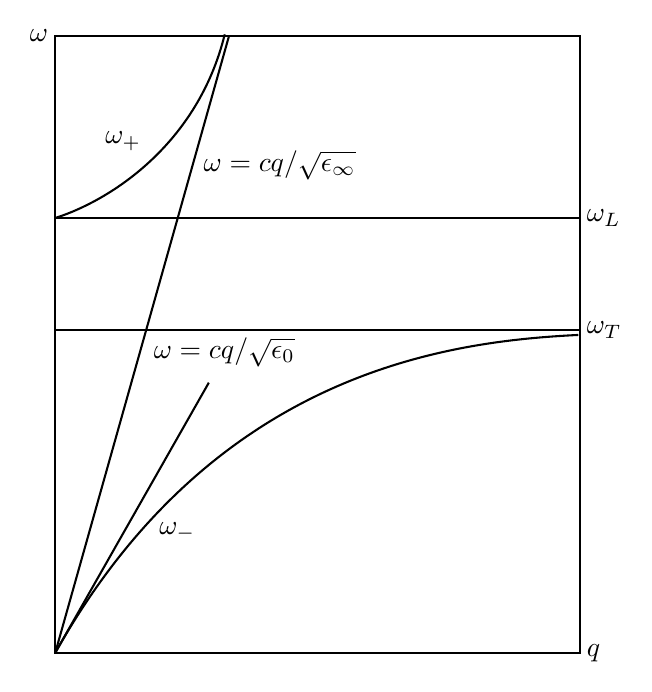
\begin{tikzpicture}[x=0.75pt,y=0.75pt,yscale=-1,xscale=1]
    %uncomment if require: \path (0,422); %set diagram left start at 0, and has height of 422

    %Shape: Rectangle [id:dp23507952836009705] 
    \draw   (100,15.5) -- (352.67,15.5) -- (352.67,312.83) -- (100,312.83) -- cycle ;
    %Straight Lines [id:da6606799809293116] 
    \draw    (100,103.33) -- (352.67,103.33) ;
    %Straight Lines [id:da5019332807627812] 
    \draw    (100,157.33) -- (352.67,157.33) ;
    %Straight Lines [id:da0033657302392038346] 
    \draw    (100,312.83) -- (183.67,15.83) ;
    %Curve Lines [id:da6548460294498928] 
    \draw    (100,103.33) .. controls (126.67,94.83) and (168.67,67.83) .. (181.67,14.83) ;
    %Straight Lines [id:da7973294821659445] 
    \draw    (100,312.83) -- (174,182.67) ;
    %Curve Lines [id:da4261274049867736] 
    \draw    (100,312.83) .. controls (177,175.67) and (292,162.67) .. (352,159.67) ;

    % Text Node
    \draw (354.67,103.33) node [anchor=west] [inner sep=0.75pt]  {$\omega _{\text{L}}$};
    % Text Node
    \draw (354.67,157.33) node [anchor=west] [inner sep=0.75pt] {$\omega _{\text{T}}$};
    % Text Node
    \draw (170,69.33) node [anchor=north west][inner sep=0.75pt] {$\omega =cq/\sqrt{\epsilon _{\infty}}$};
    % Text Node
    \draw (146,159.33) node [anchor=north west][inner sep=0.75pt] {$\omega =cq/\sqrt{\epsilon _{0}}$};
    % Text Node
    \draw (122.67,66.33) node [anchor=west] [inner sep=0.75pt] {$\omega _{+}$};
    % Text Node
    \draw (148.67,254.33) node [anchor=west] [inner sep=0.75pt] {$\omega _{-}$};
    % Text Node
    \draw (98,15.5) node [anchor=east] [inner sep=0.75pt]  {$\omega $};
    % Text Node
    \draw (354.67,312.83) node [anchor=west] [inner sep=0.75pt]  {$q$};


    \end{tikzpicture}

    \caption{横长光学波与电磁波的耦合}
\end{figure}

总之会求解得到三支谱,包括看起来没有发生什么变化的纵波模式,以及两个横波模式。
一些书上会说:“纵波模式没有和电磁波耦合,因为观察黄方程的形式,会发现只有横波模式能够和电磁波耦合,而电磁波是横波”。
这个说法是正确的,但是要说明,虽然纵波模式显然不会有通常意义上的、满足横波条件$\div{\vb*{E}}=0$的\emph{电磁波}伴随它,它仍然和\emph{电磁场}耦合,这个电磁场就是先前讨论的那个纵波模式激发出来的、产生额外回复力的库伦电场,是宏观的库伦电场,不是已经被归为“回复力”而不放进宏观的$\vb*{E}$中的那部分库伦电场。
实际上,直接将黄方程和麦克斯韦方程联立求解,由纵波条件能够严格证明$\curl{\vb*{E}}=0$;这其实说明黄方程本身的形式就蕴含了“介质激发出来的电场近似看成静电场”这一条件。
介质中的极化如果正比于$\vb*{E}$,极化就相当于只是修正了一下$\epsilon_0$,从而介质中的能够长距离传播的电磁场模式——即所谓“电磁波”——和真空中没有太大区别,横波条件总是满足的。
但在电磁波和黄方程耦合的情况下,多出来的$\vb*{W}$场可以提供不满足横波条件的$\vb*{P}$,于是仍然能有纵波和电磁场的耦合。
此时$\vb*{W}$满足纵波条件会让$\curl{\vb*{E}}=0$,因此与$\vb*{W}$耦合的电磁场基本上是静电场(准确地说是似稳场,并且没有宏观电流),正好给出先前得到的$\omega=\omega_\text{LO}$的模式。
这个模式中的电磁场虽然是宏观的,但是不能“逃逸”出晶体,因为库伦场总是局限在电荷附近的,因此它不能通过很远处产生的、在空间中走过一段距离后传入晶体的(横场的)电磁波激发,这就是我们不称它为电磁波的原因。

求解得到的另外两支谱,一支在$\vb*{k} \to 0$时,一支在$\vb*{k} \to \infty$时会展现出类似于电磁波的色散关系,但应当注意此时$\vb*{W}$始终是存在的,类似于远离共振频率的受迫振子;在介质中横光学波一定会和电磁波耦合,电磁波一定会激发出横光学波。
表面上,某一支谱在$\vb*{q} \to \infty$时存在仅有横光学波而没有电磁波的模式,但是这其实是因为电磁波频率和横光学波固有频率非常接近,从而共振导致的,此时实际上横光学波的耗散已经不能忽略了。
能够激发出这个模式的电磁波将会被强烈吸收,以及在界面处被强烈地反射。
然而,即使是在$\vb*{q} \to \infty$时,这个模式中实际上也同时有光学波(格波)和电磁波。
这些模式称为\concept{极化激元(polariton)},它们是电磁波和(与极化直接相关的横场的)光学声子的混合,属于玻色型激发。

\section{声子-声子散射}

由于实际上,晶格中的离子实之间的相互作用并不是线性的,哈密顿量中会有诸如$\vb*{X}$和$\vb*{P}$的高阶项,从而会会有${b}, {b}^\dagger$的高于二次的项,也就是说,出现了声子-声子相互作用。

不同类型的晶格中,声子-声子相互作用可能有很大的不同。

\subsection{相互作用和热膨胀}

本节分析晶格的等压热膨胀。一般来说,如果晶体表面上有压力,那么晶体内部将会出现形变且形变有梯度以产生应力来和外表面压力抵消。
换而言之,基态中$\vb*{X}$将有一个非零经典值,即处在相干态中,声子相当于处在玻色-爱因斯坦凝聚中。
然而大气压通常不会让材料有特别大的形变。因此,下面我们在宏观的热力学方程中令$p=0$(并且在求导时忽略下标$p$),而在微观模型中假定基态中晶格没有任何形变,这两个说法等价。

设没有声子时晶体体积为$V_0$。假定晶格内能主要还是由二次型的哈密顿量贡献的(通常都是如此——无论如何,Dulong-Petit定律是成立的),则根据近独立玻色子系统的热力学有
\[
    F = U + T \sum_i \left( \frac{\omega_i}{2 T} + \ln(1 - \ee^{- \omega_j / T}) \right),
\]
而
\[
    p = - \left(\pdv{F}{V}\right)_{T} = - \left(\pdv{U}{V}\right)_T - \sum_i \left( \frac{1}{2} + \frac{\omega_i}{\ee^{\omega_i / T} - 1} \right) \dv{\omega_i}{V}.
\]
我们考虑一类常见的情况,即\concept{格林爱森常数}
\begin{equation}
    \gamma = - \dv{\ln \omega_i}{\ln V}
\end{equation}
大体上不变的情况(无声子-声子散射的情况显然满足这个条件,且$\gamma = 0$)。
此时我们有
\begin{equation}
    0 = p = - \left(\pdv{U}{V}\right)_T + \gamma \frac{U}{V}.
    \label{eq:crystal-state-eq-u-v}
\end{equation}
这就给出了晶体的状态方程。设没有任何声子激发时体积为$V_0$,显然
\[
    \eval{\left(\pdv{U}{V}\right)_T}_{V_0} = 0,
\]
在这个点附近展开\eqref{eq:crystal-state-eq-u-v},有
\[
    \eval{\left(\pdv[2]{U}{V}\right)_T}_{V_0} \Delta V = \gamma \frac{U}{V},
\]
考虑到体膨胀系数的定义
\[
    \alpha = \pdv{T} \left(\frac{\Delta V}{V_0}\right)_{V_0}
\]
以及体变模量的定义
\[
    K_0 = V_0 \eval{\left(\pdv[2]{U}{V}\right)_T}_{V_0},
\]
得到
\begin{equation}
    \alpha = \frac{\gamma}{K_0} \frac{C_V}{V}.
\end{equation}
此即\concept{格林爱森关系}。

\subsection{热输运}

声子是热输运的载体之一,但不是唯一载体,如在金属中热量主要是电子输运导致的。
对声子热输运的一个粗糙的估计如下。假定声子数目不变,考虑声子平均自由程远小于晶体尺寸的情况,从而输运属于扩散,即声子流完全来自晶体内部的声子密度梯度,从而完全来自晶体内部的温度梯度。
设$c$为单电子携带的能量,则
\[
    j_\theta = - \expval*{v n c \Delta T} = - \expval{v n c \pdv{T}{x} v \tau} = - \frac{1}{3} C_V v \lambda \pdv{T}{x},
\]
即
\begin{equation}
    \vb*{j}_\theta = -\kappa \grad{T}, \quad \kappa = \frac{1}{3} C_V v \lambda.
\end{equation}
平均自由程$\lambda$的大小由很多因素确定。首先,声子-声子散射会限制声子的平均自由程。声子-声子散射有两种,其一是\concept{正规过程},即初末动量相同,另一种是\concept{Umklapp过程},其中初末动量相差一个倒格矢。
正规过程影响了动量的分布,但热流的方向大体上是不变的,而Umklapp过程会导致两个向前的声子合并后反而向后,即会导致热流方向反转,从而是主要的阻碍传热的因素。
此外,声子与杂质、缺陷、界面的散射也会影响平均自由程。

声子平均自由程和温度有非常密切的关系。在高温下,或者说$T > \omega_\text{D}$时,可以把晶格当成经典统计系统,此时
\begin{equation}
    n_{\sigma \vb*{q}} = \frac{1}{\ee^{\omega_{\sigma \vb*{q}} / T} - 1} \approx \frac{T}{\omega_{\sigma \vb*{q}}},
\end{equation}
由于$1/ \tau$正比于散射几率而散射几率正比于声子数,有
\begin{equation}
    \tau \propto \frac{1}{T} \quad \text{when $T > \omega_\text{D}$}.
\end{equation}
在低温下,即$T \ll \omega_\text{D}$时,高动量声子的数量指数衰减,于是Umklapp过程的发生几率也随之衰减,有
\begin{equation}
    \tau \propto \ee^{\omega_\text{D} / \alpha T}.
\end{equation}

\section{电子-声子耦合}

电子-声子耦合是因为电子在晶格产生的库伦势中运动。显然我们有
\[
    V \sim \int \dd[3]{\vb*{r}} \rho_\text{e}(\vb*{r}) V_\text{ion}(\vb*{r}),
\]
我们取最低阶的近似,认为$V_\text{ion}(\vb*{r})$正比于$\vb*{r}$点的离子实数密度,由于离子实并非一个理想的正电荷,而是受核外电子屏蔽的一个正电荷,离子实产生的电势随着距离上升指数衰减,因此这样假设是合理的。
于是
\[
    V \sim \int \dd[3]{\vb*{r}} \rho_\text{e}(\vb*{r}) \rho_\text{ion}(\vb*{r}).
\]
如果$\{\vb*{X}_n\}$完全没有偏离理想晶格,即晶格没有发生任何形变,那么上式实际上给出了电子质量的一个修正,可以归入电子质量项。
当晶格发生形变,但是形变很小时,根据输运方程我们有
\[
    \Delta \rho_\text{ion} \sim \div{\vb*{X}},
\]
这里我们将原本定义在格子上的$\vb*{X}$做了一个延拓,假定它在空间中是连续变化的,这是将离散的、一个一个尖峰的离子实密度连续化的常用方法。
于是,扣除了背景项(背景项导致了电子质量的修正)之后,相互作用为
\[
    V \sim \int \dd[3]{\vb*{r}} \rho_\text{e}(\vb*{r}) \div{\vb*{X}}.
\]
我们可以直接把上式量子化并切换到动量空间。
我们有
\begin{equation}
    {\rho}_{\text{e} \vb*{q}} = \sum_{\vb*{k}, \sigma} {c}^\dagger_{\vb*{k} + \vb*{q}, \sigma} {c}_{\vb*{k} \sigma},
\end{equation}
并注意到${\vb*{X}}$实际上是${b}, {b}^\dagger$的线性组合,例如对三维单成分正方晶格,我们根据\eqref{eq:transform-b-pq},得到
\begin{equation}
    {H}_\text{int} = \gamma \sum_{\vb*{q}, \lambda} \frac{\ii \vb*{q} \cdot \vu*{\lambda}_{\vb*{q}}}{\sqrt{2 M \omega_{\vb*{q} \lambda}}} ({b}_{\vb*{q} \vb*{\lambda}} + {b}^\dagger_{-\vb*{q} \vb*{\lambda}}) \sum_{\vb*{k}, \sigma}  {c}^\dagger_{\vb*{k} + \vb*{q}, \sigma} {c}_{\vb*{k} \sigma} .
    \label{eq:simple-phonon-electron-int}
\end{equation}
这里,$\gamma$是由$\rho_\text{ion}(\vb*{r})$和$V_\text{ion}(\vb*{r})$之间的关系确定的$\rho_\text{e}(\vb*{r})$和$\div{\vb*{X}}$的耦合常数,因子$\ii \vb*{q} \cdot \vu*{\lambda}_{\vb*{q}}$来自对$\vb*{X}$的散度。
于是我们就得到了二电子、一声子的相互作用,在费曼图中体现为一个二电子线一进一出、一声子线的顶角。

电子-声子散射远不止这一种类型。值得注意的电子-声子相互作用包括电子和声学声子的短程散射,极化晶体中电子和光学声子的散射等。
电子-声子散射会导致多种物理效应,包括有效电子-电子相互作用(电子交换声子产生有效电子-电子吸引)和电子弛豫(电子与热态的声子碰撞导致能量损失)等。
电子-声子散射是电阻的一个重要来源。在温度高于德拜温度时可以认为经典的能量均分定理成立,于是晶格振幅平方正比于温度,而电子-声子散射顶角通常正比于声子场的一次方,于是
\[
    \frac{1}{\tau} \propto \abs{M}^2 \propto \vb*{X}^2 \propto T,
\]
因此电阻正比于$T$。在低温下会被激发起来的声子模式数目正比于$T^3$,而。
电子在离子晶体中移动时,将让周围的正负离子产生相对位移,形成介质局域极化,即激发出光学声子,由此产生一个电子和光学声子混合的模式,称为\concept{极化子(polaron)}。
注意极化子是费米型激发,不是玻色型的极化激元。
电子-声子散射也会反过来影响声子自身的行为,如声子谱在一些点会出现强烈的扭折,这是来自这些点上强烈的电子-声子相互作用,称为\concept{Kohn反常}。
电子-声子散射导致的物理过程如此之多,我们将不在本节一一列举,而是将具体计算留到后面。

\section{局域振动}

\section{关于非晶体的振动模式}

非晶体没有晶格,也就没有晶格动量;但是非晶体当然也有振动本征模式,而且也有$3N$个。
我们仍然可以测定非晶体中的振动态密度,因为无论如何非晶体的振动都有固定的频率。
观察实验测定结果(Raman光谱,红外吸收谱等仍然可以大体反映)会发现非晶体的振动态密度通常比较光滑,这在预期之中,因为非晶体没有布里渊区,没有高对称点,自然没有态密度非常集中的地方。